\newpage
\begin{center}
    \textbf{BAB III}\\
    \textbf{METODE PENELITIAN}
    \addcontentsline{toc}{chapter}{BAB III. METODE PENELITIAN}
\end{center}

\textbf{A. Model Pengembangan}
\addcontentsline{toc}{section}{A. Model Pengembangan}


\hspace*{1cm}Penelitian ini merupakan jenis penelitian dan pengembangan (\textit{Research and Development}, R\&D). Menurut \cite{borg1989}, penelitian dan pengembangan adalah suatu proses atau metode yang digunakan untuk mengembangkan serta memvalidasi produk pendidikan. Penelitian dan pengembangan tidak hanya berfungsi untuk menghasilkan produk baru, tetapi juga untuk menyempurnakan produk yang sudah ada agar menjadi lebih praktis, efektif, dan efisien dalam penggunaannya \citep{sugiyono2018}.

\hspace*{1cm}Dalam penelitian ini, produk yang dikembangkan adalah media pembelajaran matematika berbasis simulasi 3D pada materi bangun ruang sisi datar. Pengembangan media ini memanfaatkan teknologi terkini, yaitu React sebagai library pengembangan antarmuka berbasis website dan Blender sebagai perangkat lunak untuk pembuatan objek tiga dimensi. Pemanfaatan kedua teknologi tersebut diharapkan mampu menghasilkan media pembelajaran yang interaktif, menarik, dan mudah diakses oleh peserta didik.

\hspace*{1cm}Model pengembangan yang digunakan dalam penelitian ini adalah model ADDIE (\textit{Analysis, Design, Development, Implementation, Evaluation}) yang dikembangkan oleh Dick dan Carey (1996). Model ADDIE merupakan salah satu model desain pembelajaran yang sistematis dan banyak digunakan dalam pengembangan media pembelajaran karena memiliki tahapan yang jelas dan terstruktur.

\hspace*{1cm}Model ADDIE terdiri atas lima tahapan utama, yaitu analisis kebutuhan (\textit{analysis}), perancangan (\textit{design}), pengembangan (\textit{development}), implementasi (\textit{implementation}), dan evaluasi (\textit{evaluation}). Setiap tahapan memiliki tujuan dan keluaran yang spesifik sehingga proses pengembangan dapat dilakukan secara sistematis dan terarah. Hal ini sejalan dengan pendapat \cite{gustiani2019} yang menyatakan bahwa model ADDIE mampu memastikan proses pembelajaran berjalan secara efektif dan efisien melalui tahapan yang terstruktur.

\hspace*{1cm}Selain itu, penggunaan model ADDIE juga didukung oleh berbagai penelitian yang menunjukkan efektivitasnya dalam pengembangan pembelajaran. Richey (2007) menyatakan bahwa model ADDIE memberikan kerangka kerja yang jelas bagi pendidik dan pengembang untuk merancang, mengembangkan, serta mengevaluasi program pembelajaran. Dengan adanya struktur yang sistematis tersebut, hasil pengembangan yang dihasilkan menjadi lebih optimal dan sesuai dengan kebutuhan peserta didik \citep{richey2007}.\\[1.5em]



\textbf{B. Prosedur Pengembangan}
\addcontentsline{toc}{section}{B. Prosedur Pengembangan}

\hspace*{1cm}Model ADDIE memiliki beberapa tahapan prosedur pengembangan yang ditunjukkan pada Gambar~\ref{gambar-addie} berikut.
\begin{figure}[H]
  \centering
  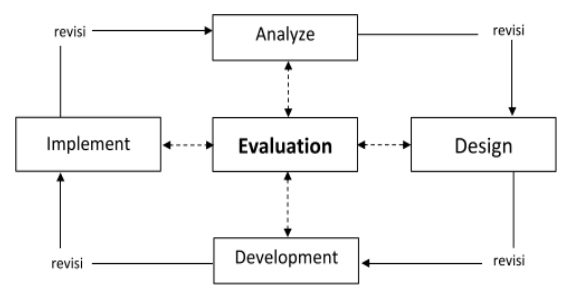
\includegraphics[width=0.8\textwidth]{images2/addie.png}
  \caption{Tahapan prosedur pengembangan model ADDIE}
  \label{gambar-addie}
\end{figure}

\hspace*{1cm}Dari Gambar~\ref{gambar-addie} di atas dapat dilihat bahwa evaluasi dilakukan di setiap akhir tahapan, bukan hanya sekali di akhir keseluruhan. Perpindahan dari satu tahapan ke tahapan selanjutnya dilakukan setelah dilakukan revisi terlebih dahulu. Berikut penjelasan dari masing-masing tahapan ADDIE yang dilakukan dalam penelitian ini.


\begin{enumerate}
    \item Analisis \textit{(Analysis)}\\
    \hspace*{1cm}Pada tahap analisis, peneliti melakukan analisis terhadap tiga hal, yaitu: analisis kebutuhan, analisis kurikulum, dan analisis karakteristik peserta didik.
    \begin{enumerate}
        \item Analisis Kebutuhan\\
        \hspace*{1cm}Pada tahap analisis kebutuhan, peneliti mengidentifikasi permasalahan yang menjadi dasar pengembangan media pembelajaran berbasis simulasi 3D. Permasalahan yang dianalisis antara lain mencakup materi yang dianggap sulit oleh peserta didik serta kebutuhan akan sumber belajar yang sudah tersedia di sekolah namun belum dimanfaatkan secara maksimal.
        \item Analisis Kurikulum\\
        \hspace*{1cm}Pada tahap analisis kurikulum, peneliti mengkaji kurikulum yang digunakan di SMP Muhammadiyah Yogyakarta serta Capaian Kompetensi yang harus dicapai oleh peserta didik, guna menentukan materi pembelajaran yang relevan untuk dikembangkan.
        \item Analisis karakteristik Peserta Didik\\
        \hspace*{1cm}Pada tahap analisis karakteristik peserta didik, peneliti melakukan observasi terhadap proses pembelajaran melalui wawancara langsung dengan pendidik kelas VIII SMP Muhammadiyah Yogyakarta. Selain itu, observasi mengenai karakteristik peserta didik juga dilakukan melalui penyebaran angket pra-penelitian menggunakan Google Form kepada peserta didik.
    \end{enumerate}
    \item Perancangan \textit{(Design)}\\
    \hspace*{1cm}Dalam proses perancangan, peneliti membagi kegiatan menjadi dua bagian: perancangan materi dan perancangan perangkat lunak. Perancangan materi dimulai dengan merumuskan tujuan pembelajaran, kemudian menyusun materi berdasarkan hasil analisis kebutuhan dan kurikulum. Perancangan perangkat lunak mencakup desain antarmuka (UI), arsitektur perangkat lunak, pembuatan model 3D, dan rancangan integrasi sistem secara keseluruhan. Peneliti juga menyusun angket validasi yang divalidasi oleh ahli dan dikoreksi oleh pembimbing.
    \newpage
    \item Pengembangan (\textit{Development})\\
\hspace*{1cm}Pada tahap pengembangan, peneliti merealisasikan desain yang telah dirancang menjadi sebuah produk berupa media pembelajaran berbasis simulasi 3D. Tahap ini bertujuan untuk menghasilkan media yang sesuai dengan kebutuhan pembelajaran serta memenuhi kriteria kelayakan. Adapun kegiatan yang dilakukan pada tahap ini meliputi:

\begin{enumerate}
\item Pembuatan Produk\\
\hspace*{1cm}Pembuatan produk diawali dengan mengimplementasikan desain yang telah disusun pada tahap sebelumnya. Kegiatan ini mencakup pengembangan antarmuka (\textit{user interface}), pembuatan model tiga dimensi menggunakan Blender, pengembangan simulasi 3D, serta perancangan sistem evaluasi pembelajaran yang terintegrasi dalam media.
\item Validasi Produk\\
\hspace*{1cm}Sebelum dilakukan uji coba, produk yang telah dikembangkan terlebih dahulu dikonsultasikan dengan dosen pembimbing untuk memperoleh masukan awal. Selanjutnya, media divalidasi oleh ahli materi dan ahli media guna mengetahui tingkat kelayakan produk. Ahli materi terdiri atas dosen Pendidikan Matematika Universitas Ahmad Dahlan dan guru matematika di SMP Muhammadiyah 9 Yogyakarta. Proses validasi ini bertujuan untuk menilai kesesuaian isi materi, tampilan media, serta aspek pembelajaran yang terdapat dalam produk.

\item Revisi Produk\\
\hspace*{1cm}Produk yang telah melalui tahap validasi selanjutnya direvisi berdasarkan saran dan masukan dari ahli materi maupun ahli media. Revisi dilakukan untuk menyempurnakan kualitas media, baik dari segi isi, tampilan, maupun fungsionalitas, sehingga produk yang dihasilkan menjadi lebih layak, menarik, dan sesuai dengan tujuan pembelajaran.

\end{enumerate}
\newpage
    \item Implementasi \textit{(Implementation)}\\
    \hspace*{1cm}Pada tahap pelaksanaan, peneliti melakukan uji coba media pembelajaran kepada peserta didik kelas VIII-B SMP Muhammadiyah 9 Yogyakarta untuk mengetahui kelayakan media yang dikembangkan. Uji coba dilakukan sebanyak dua kali, yaitu uji coba kelompok kecil dan uji coba kelompok besar. Pada setiap akhir uji coba, peserta didik diberikan angket untuk mengetahui respons mereka terhadap media pembelajaran berbasis simulasi 3D yang sedang dikembangkan.

    \item Evaluasi \textit{(Evaluation)}\\
    \hspace*{1cm}Tahap terakhir adalah evaluasi terhadap media pembelajaran yang telah dikembangkan. Pada tahap ini, evaluasi dilakukan berdasarkan hasil penyebaran angket yang telah diberikan kepada ahli materi, ahli media, serta respons dari peserta didik.\\


\end{enumerate}

\textbf{C. Uji Coba Produk}
\addcontentsline{toc}{section}{C. Uji Coba Produk}

\hspace*{1cm}Uji coba produk meliputi desain uji coba, subjek uji coba, jenis data, metode dan instrumen pengumpulan data, serta teknik analisis data. Berikut penjabaran dari masing-masing komponen tersebut.
\begin{enumerate}
    \item Desain Uji Coba\\
    \hspace*{1cm}Produk berupa media pembelajaran perlu diuji cobakan terlebih dahulu untuk mengetahui kualitas dan tingkat kelayakannya. Uji coba dalam penelitian ini dilaksanakan pada peserta didik kelas VIII-B SMP Muhammadiyah 9 Yogyakarta. Pada tahap desain uji coba, terdapat beberapa tahapan, di antaranya sebagai berikut:
    \begin{enumerate}
        \item Validasi Ahli\\
        \hspace*{1cm}Pada tahap ini, dilakukan validasi terhadap media pembelajaran yang dikembangkan oleh para ahli untuk memperoleh pertimbangan dan masukan. Hasil validasi dianalisis untuk menentukan kelayakan media. Jika media dinyatakan layak tanpa revisi, media dapat langsung diuji cobakan di lapangan. Jika diperlukan revisi, revisi dilakukan terlebih dahulu sebelum uji coba kelas kecil dilaksanakan.
        \item Uji Coba Kelas Kecil\\
        \hspace*{1cm}Setelah divalidasi oleh ahli, media diuji cobakan pada sampel peserta didik kelas VIII-B SMP Muhammadiyah 9 Yogyakarta. Uji coba ini dilaksanakan melalui pembelajaran menggunakan media. Setelah pembelajaran selesai, peserta didik mengisi angket untuk memberikan penilaian mengenai kualitas media pembelajaran berbasis simulasi 3D.
        \item Revisi Produk\\
        \hspace*{1cm}Setelah memperoleh respons dari peserta didik terkait kekurangan media pembelajaran yang dikembangkan, peneliti akan melakukan revisi apabila masih terdapat kritik dan saran yang menunjukkan perlunya perbaikan terhadap media tersebut.
        \item Uji Coba Kelas Besar\\
        \hspace*{1cm}Uji coba kelas besar dilakukan pada seluruh peserta didik kelas VIII-B SMP Muhammadiyah 9 Yogyakarta untuk mengetahui respons mereka terhadap media pembelajaran berbasis simulasi 3D yang dikembangkan. Pada tahap ini, pembelajaran dilaksanakan menggunakan media, dan di akhir pembelajaran, peserta didik mengisi angket untuk memberikan informasi mengenai kelayakan media berdasarkan pengalaman mereka.
    \end{enumerate}

    \item Subjek Uji Coba\\
    \hspace*{1cm}Subjek uji coba dalam penelitian ini terdiri dari:
    \begin{enumerate}
        \item Ahli Materi\\
        Ahli materi dalam penelitian ini adalah dosen Pendidikan Matematika Universitas Ahmad Dahlan (UAD) dan pendidik mata pelajaran Matematika kelas VIII-B SMP Muhammadiyah 9 Yogyakarta. Peran ahli materi adalah memberikan penilaian terhadap kesesuaian materi yang disajikan dalam media pembelajaran berbasis simulasi 3D yang dikembangkan.

        \item Ahli Media\\
        Ahli media merupakan dosen Pendidikan Matematika UAD dan pendidik Matematika kelas VIII-B SMP Muhammadiyah 9 Yogyakarta. Ahli media memberikan penilaian terhadap kelayakan penyajian media, termasuk aspek gambar, simbol-simbol, serta desain media pembelajaran berbasis simulasi 3D yang dikembangkan.

        \item Peserta Didik\\
        Peserta didik dalam penelitian ini adalah siswa kelas VIII-B SMP Muhammadiyah 9 Yogyakarta. Dalam uji coba media pembelajaran, peserta didik berperan sebagai responden pada tahap uji coba kelas kecil maupun kelas besar, serta memberikan tanggapan atau respons terhadap media pembelajaran berbasis simulasi 3D yang dikembangkan.
    \end{enumerate}

    \item Jenis Data\\
    \hspace*{1cm}Jenis data dikelompokkan berdasarkan sifatnya, antara lain sebagai berikut:
    \begin{enumerate}
        \item Data Kualitatif\\
        \hspace*{1cm}Data kualitatif merupakan data yang disajikan dalam bentuk pernyataan atau kalimat. Dalam penelitian ini, data kualitatif diperoleh melalui angket uji kelayakan media pembelajaran berbasis simulasi 3D yang diberikan kepada ahli materi, ahli media, dan peserta didik. Angket tersebut menggunakan skala Likert dengan lima pilihan jawaban, yaitu: Sangat Baik (SB), Baik (B), Cukup Baik (CB), Kurang (K), dan Sangat Kurang (SK).
        \item Data Kuantitatif\\
        \hspace*{1cm}Data kuantitatif merupakan data yang digunakan untuk mengukur kelayakan media pembelajaran berbasis simulasi 3D dalam bentuk angka. Dalam penelitian ini, data kuantitatif diperoleh dari hasil skor angket uji kelayakan media pembelajaran yang diberikan kepada ahli materi, ahli media, dan peserta didik. Skala penilaian yang digunakan terdiri dari lima kategori, yaitu: Sangat Baik (SB) dengan skor 5, Baik (B) dengan skor 4, Cukup Baik (CB) dengan skor 3, Kurang (K) dengan skor 2, dan Sangat Kurang (SK) dengan skor 1.
    \end{enumerate}
    \item Metode dan Instrumen Pengumpulan Data\\
    \hspace*{1cm}Metode pengumpulan data yang digunakan dalam penelitian ini meliputi wawancara dan angket untuk memperoleh data yang mendukung pengembangan media pembelajaran yang layak.
    \begin{enumerate}
        \item Instrumen Wawancara\\
        \hspace*{1cm}Wawancara merupakan salah satu metode pengumpulan data yang bertujuan untuk menemukan permasalahan yang akan diteliti serta menggali informasi lebih mendalam dari responden \citep{sugiyono2018}. Dalam penelitian ini, wawancara dilakukan terhadap pendidik mata pelajaran Matematika dan beberapa peserta didik kelas VIII-B SMP Muhammadiyah 9 Yogyakarta. Tujuan dari wawancara ini adalah untuk mengetahui berbagai permasalahan yang muncul dalam proses pembelajaran Matematika.
        \item Angket\\
        \hspace*{1cm}Angket merupakan metode pengumpulan data yang dilakukan dengan memberikan pertanyaan-pertanyaan tertulis kepada responden untuk memperoleh jawaban dari mereka \citep{sugiyono2018}. Dalam penelitian ini, instrumen angket dibagi menjadi empat jenis, yaitu sebagai berikut:
        \begin{enumerate}
            \item Angket untuk Ahli Materi\\
            \hspace*{1cm}Angket ini diberikan kepada ahli materi dengan tujuan untuk menilai kelayakan media pembelajaran berbasis simulasi 3D dari aspek materi sebelum digunakan dalam proses pembelajaran oleh peserta didik. Angket yang digunakan dalam penelitian ini menggunakan skala Likert dengan metode checklist pada setiap butir pernyataan penilaian. Kisi-kisi angket untuk ahli materi disajikan pada Tabel \ref{kisiahlimateri} berikut.
            \begin{table}[H]
                \centering
                \caption{Kisi-kisi Instrumen Angket Ahli Materi}
                \label{kisiahlimateri}
                \begin{tabular}{|c|p{2.5cm}|p{6cm}|p{3.5cm}|}
                    \hline
                    \textbf{No} & \textbf{Aspek} & \textbf{Indikator} & \textbf{Butir}\\
                    \hline
                    1 & Isi & Kesesuaian materi dengan Capaian Pembelajaran (CP) & \(1,2,3\)\\
                    & & Keakuratan materi & \(4,5,6,7,8,9\)\\
                    & & Kemutakhiran materi & \(10,11\)\\
                    & & Mendorong keingintahuan & \(12,13,14\)\\
                    \hline
                    2 & Bahasa & Penggunaan bahasa yang efektif & \(15,16\)\\
                    & & Kemampuan mendorong rasa keingintahuan peserta didik & \(17,18\)\\
                    & & Kesesuaian dengan kaidah bahasa indonesia & \(19,20\)\\
                    & & Keterbacaan & \(21\)\\
                    \hline
                    3 & Penyajian & Keruntutan penyajian & \(22\)\\
                    & & Pendukung penyajian & \(23,24,25,26,27,28\)\\
                    & & Kelengkapan penyajian & \(29\)\\
                    \hline
                    4 & Simulasi 3D & Penyampaian materi & \(30,31,32\)\\
                    \hline
                    

                \hline
                \end{tabular}
            \end{table}
            \item Angket untuk Ahli Media\\
            \hspace*{1cm}Angket ini diberikan kepada ahli media dengan tujuan untuk menilai kualitas visual dan penyajian konsep dalam media pembelajaran berbasis simulasi 3D dari aspek media. Angket yang digunakan dalam penelitian ini juga menggunakan skala Likert dengan metode checklist pada setiap butir penilaian. Kisi-kisi angket untuk ahli media disajikan pada Tabel \ref{kisiahlimedia} berikut.
            \begin{table}[H]
                \centering
                \caption{Kisi-kisi Instrumen Angket Ahli Media}
                \label{kisiahlimedia}
                \begin{tabular}{|c|p{3.5cm}|p{5.5cm}|p{4.5cm}|}
                    \hline
                    \textbf{No} & \textbf{Aspek} & \textbf{Indikator} & \textbf{Butir}\\
                    \hline
                    1 & Kualitas kegrafikan & Ukuran media pembelajaran & \(1,2\)\\
                    && Desain isi media pembelajaran & \(3,4,5,6,7,8,9,10,11,12\)\\
                    \hline
                    2 & Kelayakan bahasa & Lugas, komunikatif, dialogis, dan interaktif & \(13,14,15,16\)\\
                    && Kesesuaian dengan perkembangan peserta didik & \(17,18,19,20\)\\
                    && Kesesuaian dengan PUEBI & \(21,22\)\\
                    && Penggunaan istilah dan simbol & \(23,24\)\\
                    \hline
                    3 & Kualitas perangkat lunak & & \(25,26,27,28,29,30\)\\
                    \hline
                    
                \end{tabular}
            \end{table}
            \item Angket Respons Peserta Didik\\
            \hspace*{1cm}Angket ini diberikan kepada peserta didik untuk mengetahui tanggapan mereka terhadap media pembelajaran berbasis simulasi 3D. Tanggapan yang diperoleh dari peserta didik digunakan sebagai acuan dalam pengembangan dan penyempurnaan media pembelajaran. Kisi-kisi angket untuk peserta didik disajikan pada Tabel \ref{kisiresponsiswa} berikut.
            \begin{table}[H]
                \centering
                \caption{Kisi-kisi Angket Respon Peserta Didik}
                \label{kisiresponsiswa}
                \begin{tabular}{|c|p{3cm}|p{6.5cm}|}
                    \hline
                    \textbf{No} & \textbf{Indikator} & \textbf{Butir}\\
                    \hline
                    1 & Penyajian Materi & \(1,2,3,4,5,6,7,8,9,10,11, 12,13,14\)\\
                    2& Tampilan & \(15,16,17,18,19,20,21\)\\
                    3& Manfaat & \(22,23,24\)\\
                    4& Ketertarikan & \(25,26\)\\
                    \hline

                    
                \end{tabular}
            \end{table}
        \end{enumerate}
    \end{enumerate}
    \item Teknik Analisis Data\\
    \hspace*{1cm}Penelitian ini menggunakan teknik analisis data untuk menentukan kelayakan media pembelajaran yang dikembangkan berdasarkan penilaian ahli materi, ahli media, dan respons peserta didik. Teknik analisis data dalam penelitian ini dilakukan melalui beberapa tahapan, yaitu:
    \begin{enumerate}
        \item Kuantitatif Data\\
        \hspace*{1cm}Data yang diperoleh dari hasil angket yang diberikan kepada ahli materi, ahli media, dan peserta didik merupakan data kualitatif yang kemudian dikonversi menjadi data kuantitatif menggunakan skala Likert. Konversi ini dilakukan berdasarkan ketentuan skor penilaian yang disajikan pada Tabel \ref{likert} berikut.
        \begin{table}[H]
            \centering
            \caption{Skala Likert}
            \label{likert}
            \begin{tabular}{|p{5cm}|c|}
                \hline
                \textbf{Kategori Penilaian} & \textbf{Skor}\\
                \hline
                Sangat Baik (SB) & 5\\
                Baik (B) & 4\\
                Cukup Baik (CB) & 3\\
                Kurang (K) & 2\\
                Sangat Kurang (SK) & 1\\
                \hline
            \end{tabular}
        \end{table}
        \item Menghitung Nilai Rata-rata\\
        \hspace*{1cm}Dari data yang sudah dikumpulkan, kemudian dihitung nilai rata-ratanya dengan menggunakan rumus sebagai berikut:
        \begin{equation}
            \bar{x}=\frac{\sum x}{n}
        \end{equation}
        \textbf{Keterangan:}\\
        \( \begin{array}{lcl}
            \bar{x} & = & \text{Nilai rata-rata}\\
            \sum x & = & \text{Jumlah seluruh skor}\\
            n & = & \text{Jumlah responden atau butir pernyataan}
        \end{array} \)

        % \( \bar{x} = \text{Nilai rata-rata} \)\\
        % \( \sum x = \text{Jumlah seluruh skor} \)\\
        % \( n = \text{Jumlah responden atau butir pernyataan} \)

        \item Klasifikasi Penilaian\\
        \hspace*{1cm}Setelah mengetahui rata-rata yang diperoleh, kemudian data tersebut diubah menjadi data kualitatif sesuai kriteria penilaian ideal. Hasil analisis data yang telah diperoleh dijadikan dasar untuk mengetahui kualitas media pembelajaran. Kriteria penilaian ideal dapat dilihat dalam Tabel \ref{kriteriaskala5} berikut ini, tabel bersumber dari buku Evaluasi Program Pembelajaran \citep{widoyoko2014}.
        \begin{table}[H]
            \centering
            \caption{Kriteria Penilaian Ideal Skala 5}
            \label{kriteriaskala5}
            \begin{tabular}{|c|p{3cm}|}
                \hline
                \textbf{Interval} & \textbf{Kriteria}\\
                \hline
                \( \bar{x} > M_i + 1{,}8~SB_i \) & Sangat Baik\\
                \( M_i + 0{,}6~SB_i < \bar{x} \leq M_i + 1{,}8~SB_i \) & Baik\\
                \( M_i - 0{,}6~SB_i < \bar{x} \leq M_i + 0{,}6~SB_i  \) & Cukup Baik\\
                \( M_i - 1{,}8~SB_i < \bar{x} \leq M_i - 0{,}6~SB_i \) & Kurang\\
                \( \bar{x} \leq M_i - 1{,}8~SB_i \) & Sangat Kurang\\
                \hline
            \end{tabular}
        \end{table}
        \textbf{Keterangan:}\\
        \( \begin{array}{lcl}
            M_i \text{ (Rata-rata ideal)} & = & \frac{1}{2} \times (\text{Skor Maksimal Ideal} + \text{Skor Minimal Ideal})\\
            SB_i \text{ (Simpangan baku ideal)} & = & \frac{1}{6} \times (\text{Skor Maksimal Ideal} - \text{Skor Minimal Ideal})\\
            \bar{x} & = & \text{Skor kevalidan}\\
            \text{Skor Maksimal Ideal} & = & \text{Jumlah Butir Kriteria} \times \text{Skor Tertinggi}\\
            \text{Skor Minimal Ideal} & = & \text{Jumlah Butir Kriteria} \times \text{Skor Terendah}
        \end{array} \)

        \item Analisis Kelayakan\\
        \hspace*{1cm}Kelayakan media pembelajaran berbasis simulasi 3D ditentukan berdasarkan hasil penilaian dari ahli materi, ahli media, dan respons peserta didik. Media pembelajaran dinyatakan layak apabila hasil penilaian berada pada kategori minimal "Baik (B)". Dengan demikian, media pembelajaran berbasis simulasi 3D tersebut layak digunakan dalam proses pembelajaran matematika di kelas VIII SMP untuk materi bangun ruang sisi datar.
    \end{enumerate}

\end{enumerate}

